The amazon dataset was the first mandatory dataset. We accomplished getting a score of 72.8\% on kaggle. It is high dimensional and has quie a lot of samples. It is not well known. Feature selection should can be used to improve results by about 20-40 percent depending on the classifier. Scaling is not that important.

\subsection{Characteristics}

\begin{itemize}
\item No missing values
\item 50 different target classes
\item Only rational data
\item 10 000 attributes
\item 750 samples
\end{itemize}

\subsection{}
As seen in Figure \ref{fig:amazon-target} there are only little samples per class.

\begin{figure}[H]
  \begin{center}
    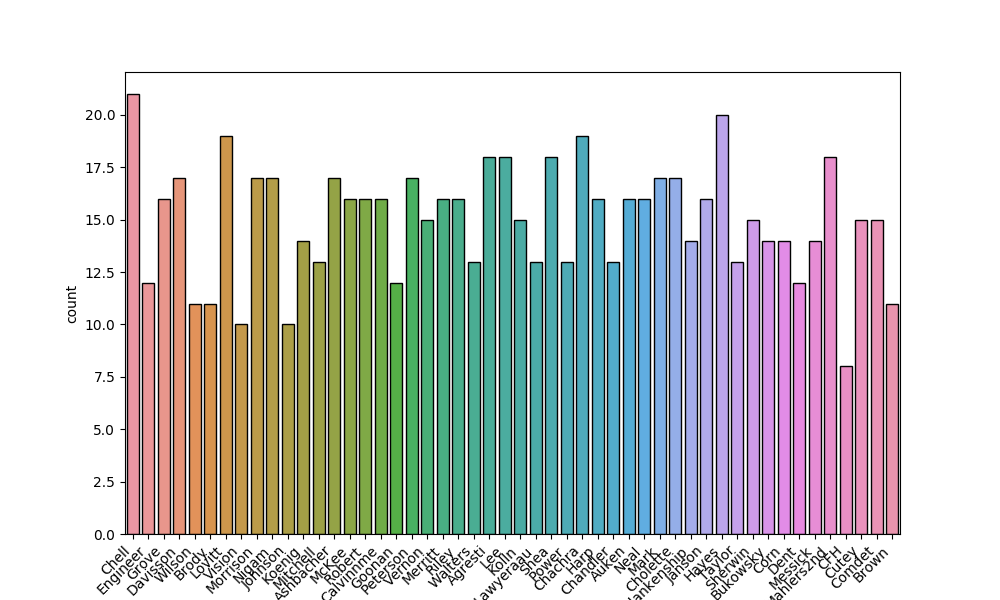
\includegraphics[width=\linewidth]{amazon/plots/target.png}
    \caption{Histogram of the target values}
    \label{fig:amazon-target}
  \end{center}
\end{figure}


\subsection{Feature selection}

We selected features based on SelectKBest, which perform ${\chi}^2$ test to the samples to retrieve the best features. We also used Recursive feature elimination with cross-validation. As seen in Figure \ref{fig:amazon-feature-selection} at least 1000 features should be used to cross the 55 percent mark, however no difference in performance could be detected between 1000 and 4000 selected features.

\begin{figure}[H]
  \begin{center}
    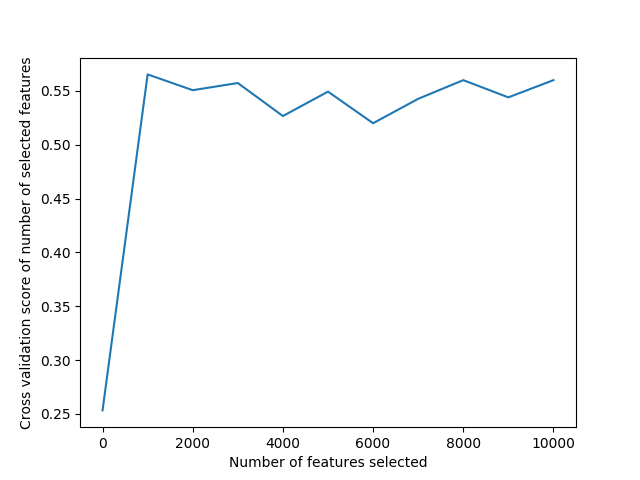
\includegraphics[height=7cm]{amazon/plots/rf_feature_selection.png}
    \caption{Comparison of different metrics}
    \label{fig:amazon-feature-selection}
  \end{center}
\end{figure}

\subsection{K Nearest Neighbors Classifier}

K Nearest Neighbors Classifier worked best with weights set to distance. Meaning that the importance of the k neighbors are weighted by their distance. This increased results by about 10\%. As seen in Figure \ref{fig:amazon-knn-metric-comparison} the manhattan metric worked best.

\begin{figure}[H]
  \begin{center}
    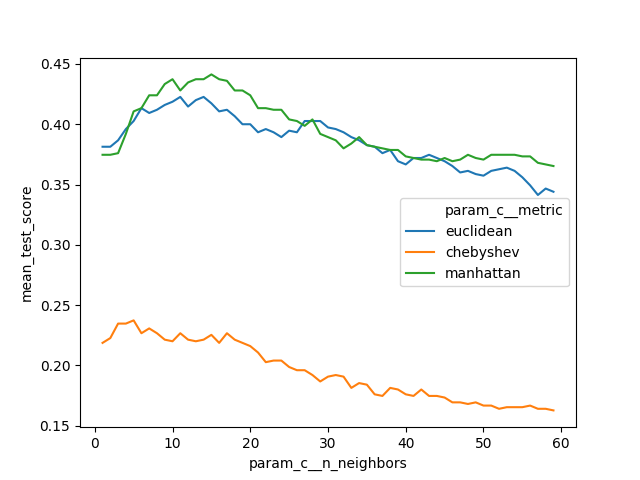
\includegraphics[width=\linewidth]{amazon/plots/knn_metrics.png}
    \caption{Comparison of different metrics}
    \label{fig:amazon-knn-metric-comparison}
  \end{center}
\end{figure}

Preprocessing with MinMax scalar improved results by around 5\% as seen in figure \ref{fig:amazon-knn-comparison}. Scaling with mean and variance did lead to better results, but it was not as good as the min max scaler.

\begin{figure}[H]
  \begin{center}
    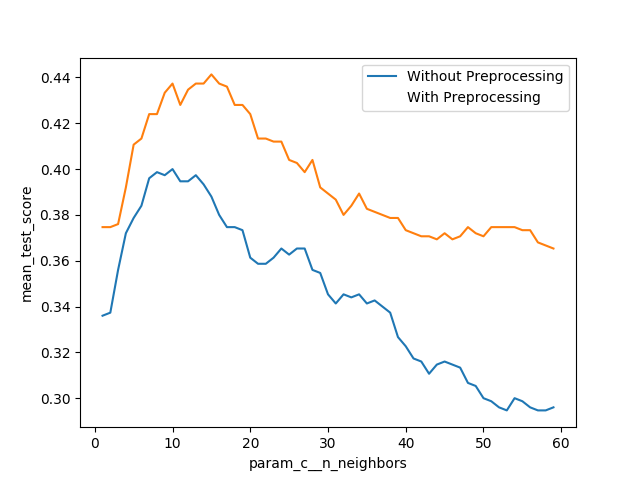
\includegraphics[width=\linewidth]{amazon/plots/knn_comparison.png}
    \caption{Comparison of the best estimators with preprocessing and without preprocessing}
    \label{fig:amazon-knn-comparison}
  \end{center}
\end{figure}


\subsection{Random Forest Classifier}

The best features of Figure \ref{fig:amazon-feature-selection} were used for the Random Forest Classifier. As seen in Figure \ref{fig:amazon-rf-comparison}, a low maximum features yielded good results. We tested different parameters for the minimum samples that lead to splitting and found out that 0.01 works well.

\begin{figure}[H]
  \begin{center}
    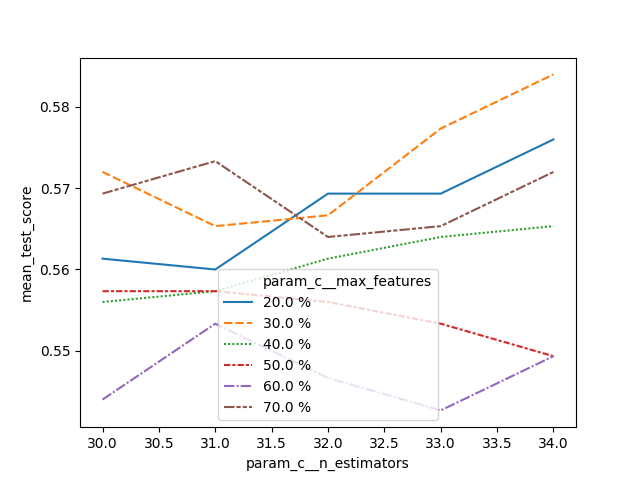
\includegraphics[width=\linewidth]{amazon/plots/rf_comparison.png}
    \caption{Comparison of the best estimators with preprocessing and without preprocessing}
    \label{fig:amazon-rf-comparison}
  \end{center}
\end{figure}

\subsection{Multi-Layer Perceptron Classifier}

Testing out different hyperparamethers for mlp takes quite a lot of time. We were able to get a score of 72 \% accuracy on kaggle by using 2000 selected features with ${\chi}^2$ tests, relu as activation and one hidden layer with 100 neurons. As shown in figure \ref{fig:mlp-comparison} choosing different activation function does not make any difference.

\begin{figure}[H]
  \begin{center}
    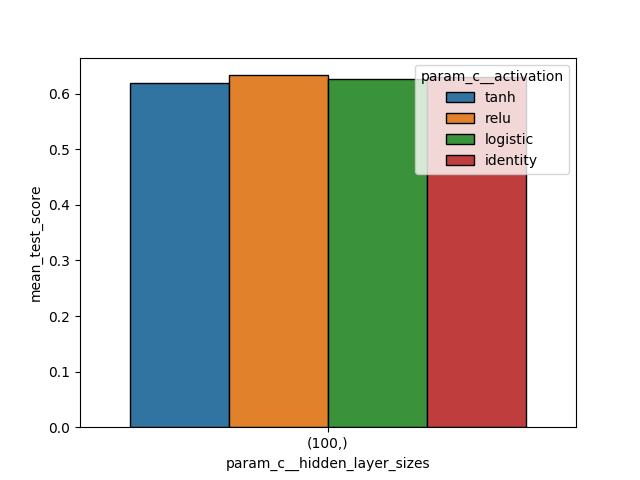
\includegraphics[width=\linewidth]{amazon/plots/mlp_comparison.png}
    \caption{Comparison of the best estimators with preprocessing and without preprocessing}
    \label{fig:mlp-comparison}
  \end{center}
\end{figure}

\subsection{Conclusion}



\begin{table}[H]
\begin{center}
\begin{tabular}{|l|l|l|}
\hline
                       & Preprocessing & No-Preprocessing \\ \hline
KNeighborsClassifier   & 0.4413        & 0.4000           \\ \hline
RandomForestClassifier & 0.6026        & 0.5840           \\ \hline
MLPClassifier          & 0.9666        & 0.9866           \\ \hline
\end{tabular}
\caption{Comparision of accuracy of different techniques with- and without preprocessing}
\end{center}
\end{table}

\begin{table}[H]
\begin{center}
\begin{tabular}{|l|l|l|}
\hline
                       & Holdout & Cross Validation \\ \hline
KNeighborsClassifier   & 0.9333  & 0.9800           \\ \hline
RandomForestClassifier & 0.9666  & 0.9666           \\ \hline
MLPClassifier          & 1.0000  & 0.9866           \\ \hline
\end{tabular}
\caption{Comparision of accuracy of holdout versus cross-validation}
\end{center}
\end{table}

\begin{table}[H]
\begin{center}
\begin{tabular}{|l|l|l|l|l|l|}
\hline
                       & Accuracy & Precision & Recall & F1     & Runtime (sec) \\ \hline
KNeighborsClassifier   & 0.4333   & 0.3847    & 0.4356 & 0.3805 & 30.987        \\ \hline
RandomForestClassifier & 0.9600   & 0.9644    & 0.9600 & 0.9597 & 0.1947        \\ \hline
MLPClassifier          & 0.9800   & 0.9848    & 0.9800 & 0.9793 & 1.5557        \\ \hline
\end{tabular}
\caption{Comparision of different performance metrics and runtimes}
\end{center}
\end{table}

